\section{Introduction}

The increase in informal housing is a common issue faced by nations globally.
Although informal regions of housing, such as slums, are commonplace in
underdeveloped countries, it affects the developed world as well, e.g., refugee
camps. Informal settlements might be difficult to monitor merely on the usage
of ground surveys due to scale, distribution or a varity of other difficulties.
Satellite and aerial images provide a solution to the problems encountered with
ground based methods.  High resolution images allow for the detection of
informal housing based exclusively on features extracted from the image.  The
images could be annotated manually although the feasability diminishes with
increased scale.  As a solution, the detection of informal settlements can be
automated using inherent visual characteristics of a certain area. The features
extracted images provide a distinct difference between formal and informal
housing. The features that are determined distinctive can used by classification
algorithms, effectively automizing the detection of areas containing informal
housing in images.

\subsection{Related works and contributions}

There are multiple studies that have researched methods for the detection of informal
housing using satellite and aerial images in the last decade \cite{kuffer2016slums}.
Informal regions in the proximity of cities have been studied throughout
the globe, e.g. Colombo \cite{colombo},
Johannesburg \cite{williams2016automatic}, Accra \cite{accra}, Mumbai
\cite{mumbai}, and Hyderabad \cite{hyderabad}. There are numerous
characteristics that are suitable to differentiate between formal and informal
areas. This could be the presence of vegetation, the width of
the roads, the size and orientations of dwellings, together with many different
methods \cite{owen2013approach}.

Due to the increase in availability of remote sensing high resolution imagery, it became
feasible to distinguish individual objects on a large scale.  This allows for
the interpretation of geographical imagery with individual objects at its
basis.  As a result, the characterization of regions may be based on the type
of objects that inhabit it.  To illustrate, a study classified rooftop objects
from aerial imagery of an informal settlements in Johannesburg to gather
demographic information as an alternative to traditional ground based survey
\cite{williams2016automatic}.

A study from 2012 conducted by Graesser \textit{et al.} characterized formal
and informal neighborhoods \cite{graesser2012image}. This paper proposed
a method for the detection of informal regions using a set of different
features extracted from satellite images. The methods for feature extraction
used where GLCM, HoG, Lacunarity, LFD, LSR, NDVI, SIFT, and TEXTON. The
features produced from these methods were able to succesfully characterize the
two types of neighborhoods.

\subsection{Proposed Method}

Our study continues with the work performed by Graesser \textit{et al.}.
A part of the research will evaluate if the results obtained by Graesser
\textit{et al.} translates to a different cities and satellite images. Beyond
the replication and evaluation of previous research, the methods of feature
extraction used by Graesser will be extended by an additional new method. The
features created from this method will be compared to the existing features.
The features extracted from the various method are combined and used by a set
of different classification algorithms to both assess the performance of the
feature set as well as the evaluation of various classification algorithms.

The paper of Graesser \textit{et al.} uses blocks of pixels instead of each
individual pixel when extracting features from images.  This is to ease the
computational load because several of the extraction methods used are
computationally quite expensive. These blocks of pixels are of 20 by
20 pixels in the paper. The size of these pixel blocks will from this part on
be refered to as the \textit{block size}. The block size will differ from
this value to evaluate the affect to the performance of the features.
In addition to blocks, the paper also uses a set of different scales for the
calculation of features. A scale specifies the pixels around a block that
are used for the calculation of that block. This allows blocks to be more
spatially connected to the surrounding areas, which can increase the
performance of a feature.

\subsection{Data}

The image data is captured by the earth observation satellite WorldView3 owned
by DigitalGlobe. The WorldView3 satellite produces multiple types of images
with varying degrees of resolution. The panchromatic images have a resolution
of 0.31 meter in contrast to  the multiband images have a significantly lower
resolution of 1.24 meter. The project uses pansharpened images, which combines
the high resolution panchromatic- and the low resolution multiband images to
create high resolution RGB images.

The content of the images contain regions of Bangalore, which is the capital
city of the indian state of Karnataka, located in south central India. The
population of the city is over ten million and is categorized as a mega city.
Banglore is known to have problems concerning informal settlements. According
to a report from 2012, there were 862 reported slums in the city

% TODO find source of slum report ^

\begin{figure}
  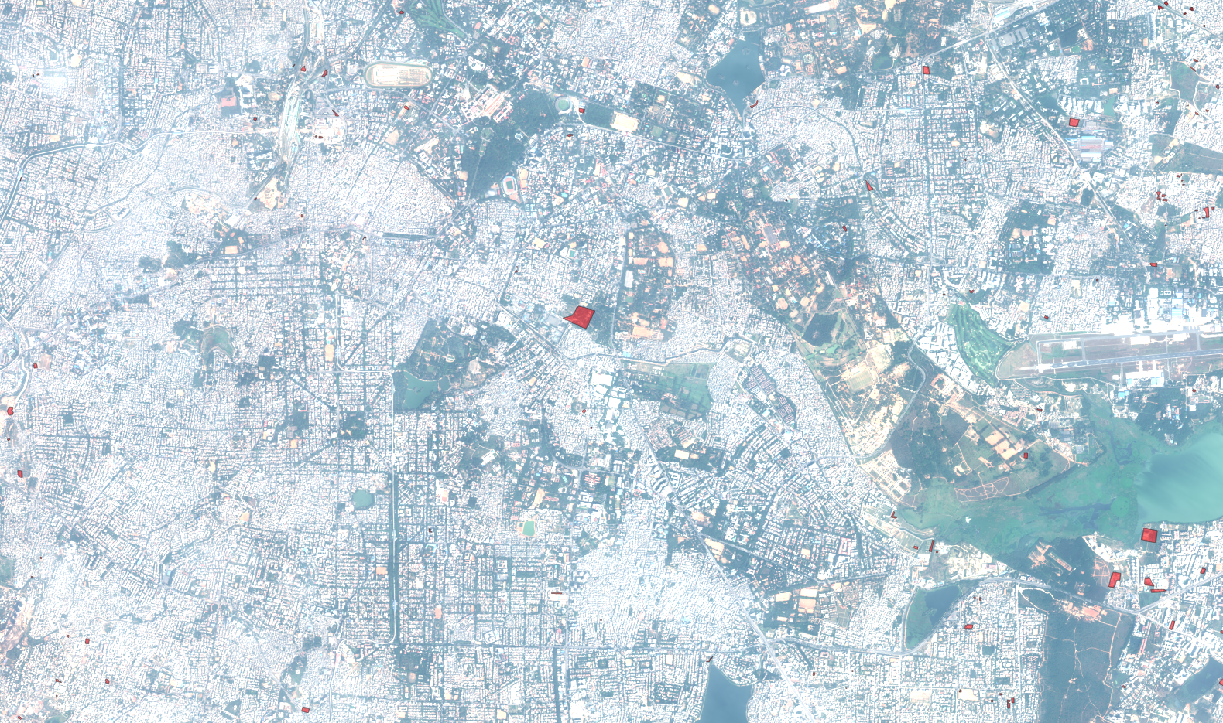
\includegraphics[width=\linewidth]{images/west-bangalore}
  \caption{A part of western Bangalore, the red patches indicate informal
  settlements}
  \label{fig:west-bangalore}
\end{figure}

\subsection{Challenges}

The distinction between formal and informal regions is often quite challenging,
in part due to the vagueness of borders between the regions. The border between
formal and informal regions often resembles more of a spectrum than a clear cut line.
Besides border difficulties, some areas are not designated as informal, while
still posessing characteristics of an informal region. This results in
a dataset with noise and inconsistency.  All in all, the binary classification
of a region encounters difficulties when applied in practice. 

Another challenge encountered in this field is the scarcity of informal
settlements.  Eventhough Banglore  has an abundance of informal settlements,
the fast majority of land is identified as formal area's. Figure
\ref{fig:west-bangalore} shows a part of western Bangalore where it is clear
that informal settlements are sparce and distributed throughout the city. As
a result, the dataset of formal and informal regions becomes quite skewed.
Furthermore, because everything that is not informal is automatically
considered formal, the formal regions have a large amount of variance of visual
properties.  To illustrate: lakes, forrests, and fields fall in the same
catagory as formal residential and industrial areas while the visual
characteristics are significantly different. The diverse content of the formal
set of visual characteristics might hinder the effectiveness of differentiating
between formal and informal regions. 

To reduce the skewedness between informal and formal, only subsections of
Figure \ref{fig:west-bangalore} are used where the proportion formal to
informal is less one-sided. The sections together with their position in the whole image, are displayed in Figure \ref{fig:sections}. A smaller difference in formal informal ratio allows for
a better understanding of the effectiveness of various features. The features
are assesed using these area's 

%\begin{figure}
%\centering
%  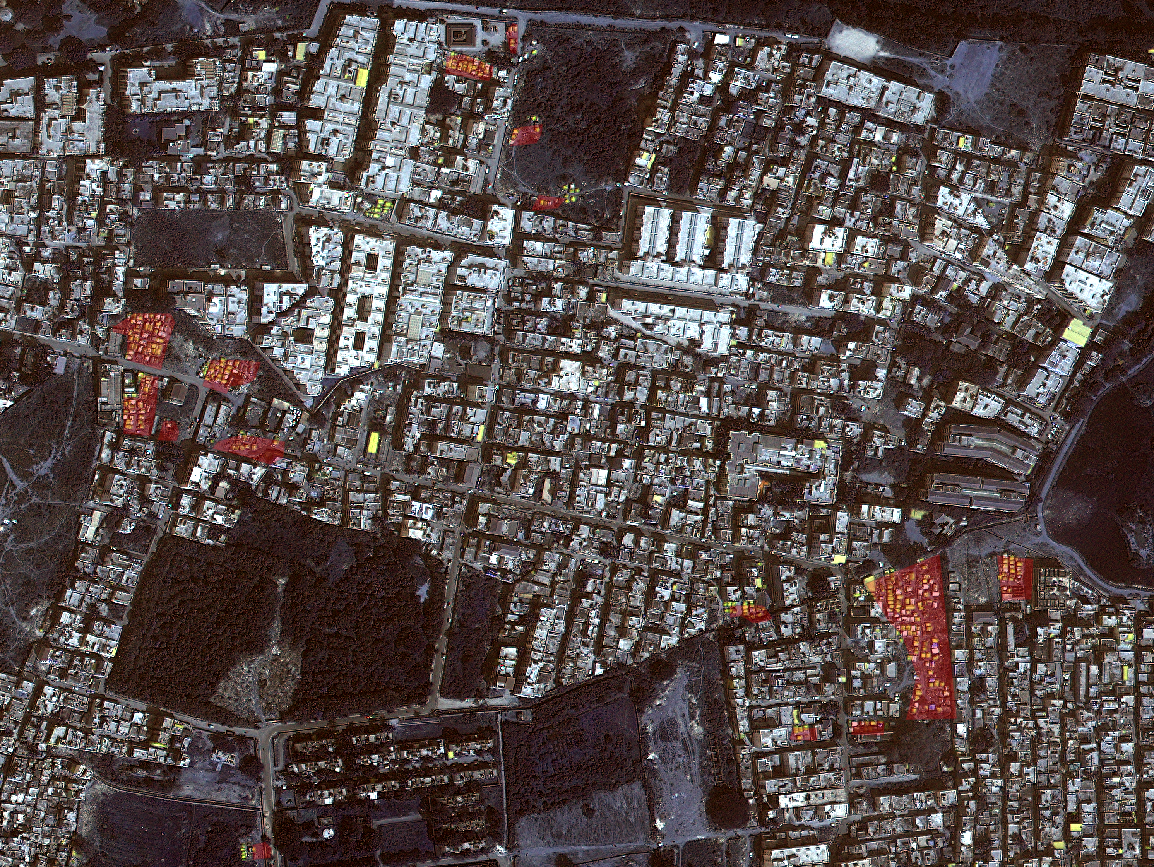
\includegraphics[width=\linewidth]{images/section_3}
%  \caption{Dense informal area in Bangalore, the red patches indicate informal
%  settlements}
%  \label{fig:section_3}
%\end{figure}


\begin{figure}
\begin{tabular}{cc}
  \subfloat[Section 1]{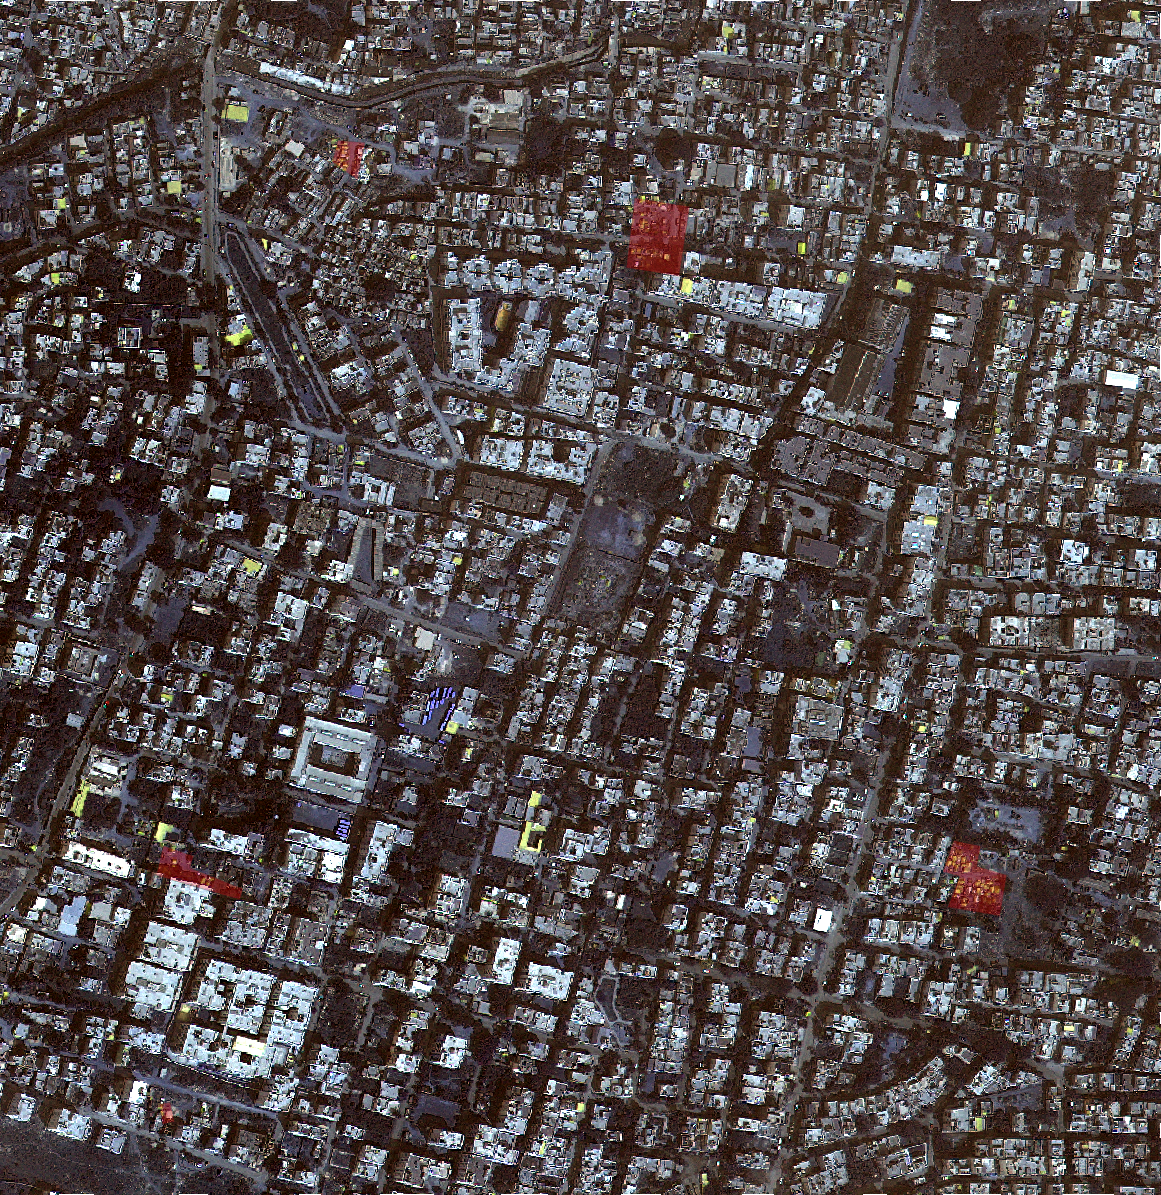
\includegraphics[width=4cm]{images/section_1}}&
  \subfloat[Section 2]{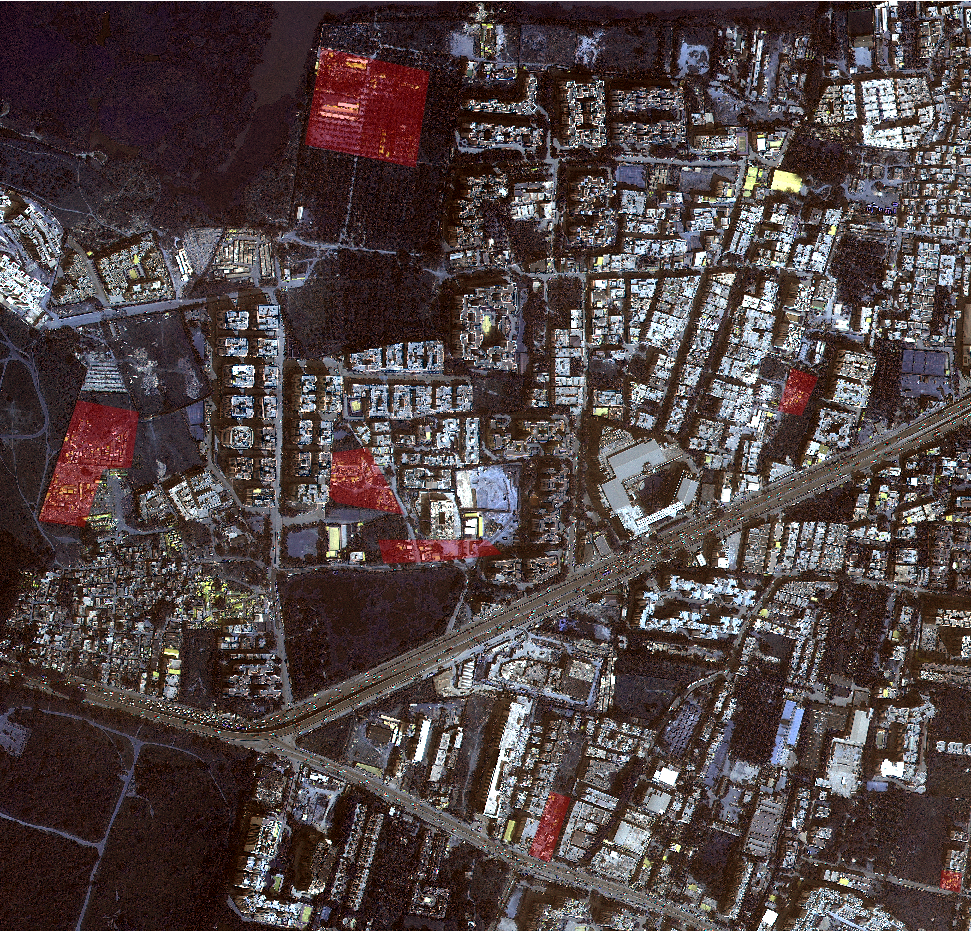
\includegraphics[width=4cm]{images/section_2}}\\
  \subfloat[Section 3]{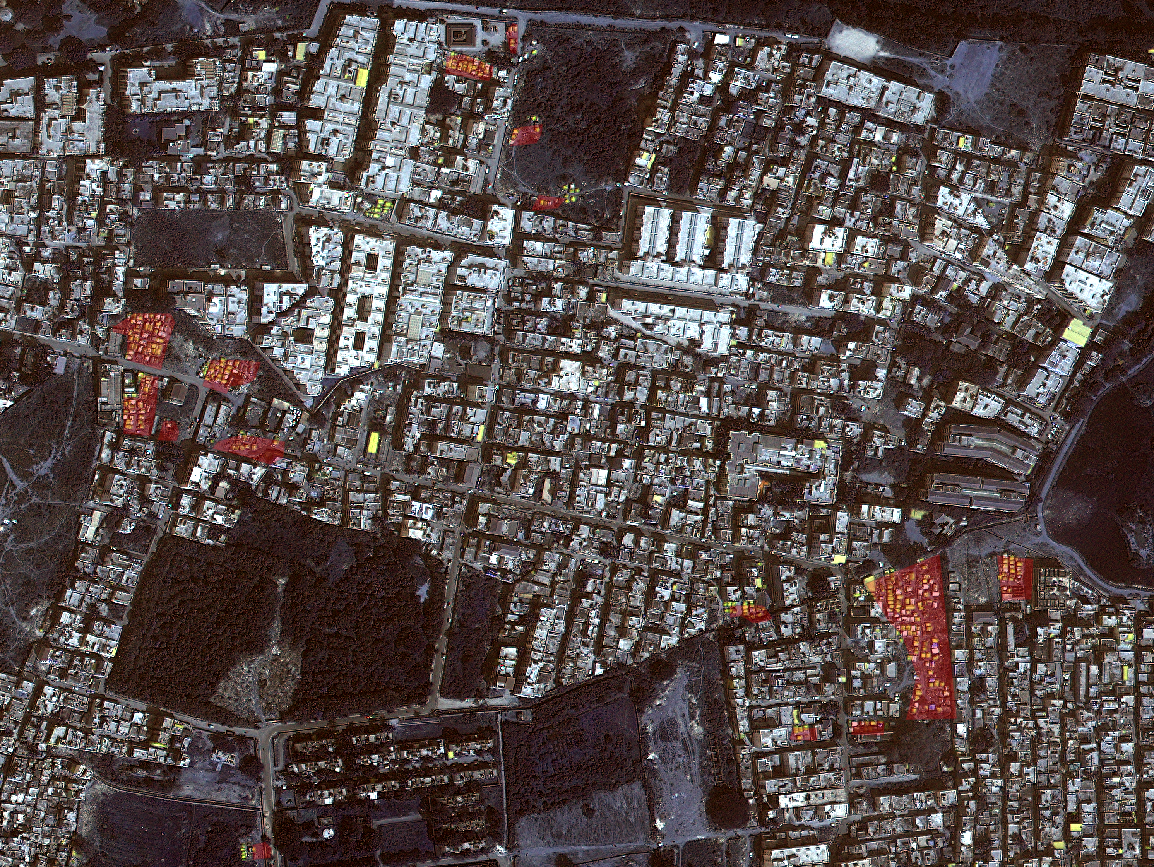
\includegraphics[width=4cm]{images/section_3}}&
  \subfloat[Location of Sections]{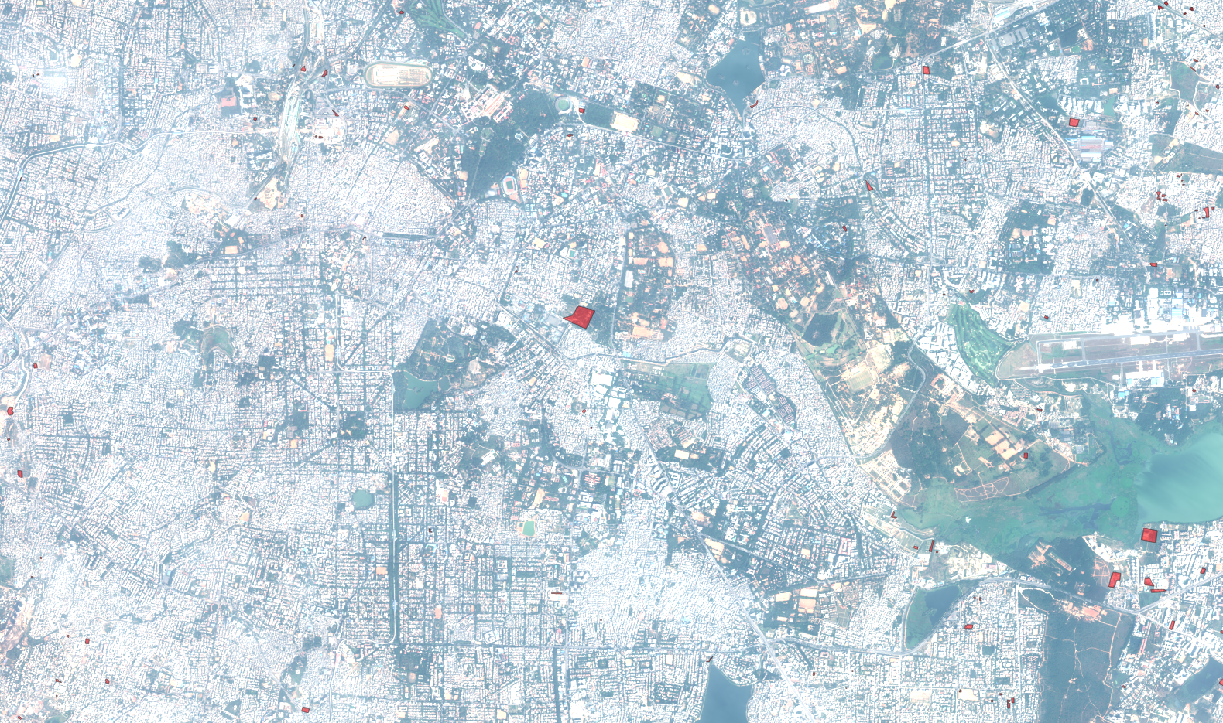
\includegraphics[width=4cm]{images/west-bangalore}}
\end{tabular}
\caption{The images used for evaluation and classification}
\label{fig:sections}
\end{figure}

